\documentclass{article}
\usepackage{hyperref}
\usepackage{graphicx}
\usepackage{algorithm2e}

\begin{document}

\title{Raising \emph{Anopheles} hybrids}

\author{Erik Garrison}

\maketitle

\begin{abstract}
In this rotation I attempted to hybridize various species in the \emph{Anopheles gambiae} species complex, with the objective of eventually applying RNA sequencing to hybrid offspring to determine if particular features of gene regulation might be result from hybrid incompatibility.
\end{abstract}


\section{Hybrid incompatibility}

An understanding of the genetics of malarial vector species of \emph{Anopheles} is an important component of malarial eradication programs \cite{pmid25554792}. The major African vector, \emph{Anopheles gambiae} is a species complex formed of two main subspecies (labeled M and S) that appear to exist in near-total reproductive isolation  \cite{lanzaro2013speciation}.
This reproductive isolation has led to the suggestion that the complex may present an example of ongoing speciation, and recently the M and S forms have been reclassified as separate species, \emph{An. gambiae sensu stricto} (S form) and \emph{An. coluzzii} (M form) \cite{pmid26131476}.
These forms, as well as other \emph{Anopheles} species, can hybridize, but following Haldane's rule, males (which are the heterogametic sex) are sterile. In the case of \emph{An. gambiae s.s.} and \emph{An. arabiensis} QTL mapping suggests that this effect results from incompatibilities between loci on the X chromosome and the autosomes \cite{slotman2004genetics}.
In the interest of better-understanding the genomics of this incompatibility, we attempted to cross various laboratory-adapted \emph{Anopheles} strains. Several crosses eventually yielded adult mosquitoes which have been retained for possible RNA sequencing and analysis.

\section{Methods}

Five laboratory strains of mosquitoes were raised from eggs purchased from a supplier:

\begin{itemize}
\item \emph{An. arabiensis} ``KGB'' (subsaharan Africa)
\item \emph{An. merus} ``merus'' (brackish, coastal)
\item \emph{An. quadrimaculatus} ``quad'' (North American)
\item \emph{An. coluzzii} ``mali-NIH'' (formerly M form)
\item \emph{An. gambiae s.s.} Pimperena ``pimp'' (formely S form).
\end{itemize}

We attempted several rounds of crossing. For each round we followed the same procedure to rear the mosquitoes. Eggs were deposited (``floated'') in net-covered trays filled with several centimeters of water containing dissolved salts and minerals typical of ponds where \emph{Anopheles} larvae are found. Larvae were fed with two kinds of fish food (liquifry and pellet) and monitored for developmental progress. Adults were collected immediately after hatching from the final larval stage. Speedy collection ensures that mating between pairs of the same species does not occur. Males are not capable of mating for several hours after hatching as the clasping apparatus that is essential for grasping the female genitalia is not functional. We attempted to collect more males than females where there was an excess of adults, aiming for approximately 3 males for every female (30 males and 90 females each), however this was not always possible.

Once collected, males and females were sorted by sex (which can be done easily with the aid of a dissecting microscope due to the distinct morphology of the sexes) and males and females of different species were placed in cages with glucose food. After several days, females were fed using donor blood placed in a petri dish covered in parafilm and heated to near human body temperature using warm water, however ``pimp'' females required live feeding on human donors. After another 24 to 48 hours, dishes with the same water used to raise larvae were placed in the cages to receive eggs. When a first feeding produced no eggs, a second round of feeding was attempted. In one case anestitized mice were used.

The objective of the rearing of these mosquito hybrids was to apply RNA sequencing to reciprocal crosses in order to find potential hybrid incompatibility QTLs. As such, we observed which crosses laid eggs, and only transferred eggs where both male-female and female-male crosses from a pair of species had laid. Adults were collected from hatching trays and placed into temporary collection cages. After hatching was complete, F1s were culled and prepared for RNA extraction by anesthetization with CO$_{2}$ and freezing at -20 °C under RNALater buffer in individually-labeled eppendorf tubes.

\section{Results}

The results of attempted crosses are listed in table \ref{tab:crosses}. In the first phase crosses between quad, merus, and kgb resulted in eggs laid in all crosses involving quad males. We hypothesize that this resulted from the fact that the \emph{An. quadrimaculatus} colony had been established in the lab for several generations before the crosses were set up, however the reasons are not clear and a second attempt was not made. Although eggs were laid in a reciprocal cross between merus and quad, very few eggs were laid in the merus male / quad female cross, and further none of the floated eggs resulted in viable larvae. It is possible that the females in these crosses were not fertilized, as sterile mating is known to result in egg laying \cite{thailayil2011spermless}. On the other hand, crosses between mali-NIH (\emph{An. coluzzii }) and pimp (\emph{An. gambiae s.s.}) reliably produced viable adult offspring, although at very low rates relative to the pure species colonies. The handful of adults that resulted from the pimp/mali-NIH crosses (see \ref{fig:malimalepimpfemale} and \ref{fig:pimpmalemalifemale}) were collected and frozen for later use. The mali-NIH male / pimp female cross resulted in 4 females and 2 males, while the reverse cross yielded only females. The number of harvested F1 adults was too small to enable further analysis on the basis of sex.

\section{Conclusion}

In this project I completed what could be considered a small pilot of a more extensive hybridization experiment. I found the work very engaging, but do not feel it is justifiable to take the samples I collected forward for sequencing and analysis.

A more rigorous study would require larger sample sizes and a complete set of crosses. If the experiment were repeated, I would begin by maintaining colonies of the pure species inputs for at least several generations so that they could habituate to the particular conditions in the insectory.

\begin{table}[]
\centering
\begin{tabular}{|l|l|l|l|l|l|}
\hline
           & quad M  & merus M  & kgb M  & mali-NIH M & pimp M     \\ \hline
quad F     & x,e,l,a  & xe      & x       &           &            \\ \hline
merus F    & x,e      & x,e,l,a & x       &           &            \\ \hline
kgb F      & x,e      & x,e     & x,e,l,a &           &            \\ \hline
mali-NIH F &          &         &         & x,e,l,a   & x,e,l,a    \\ \hline
pimp F     &          &         &         & x,e,l,a   & x,e,l,a    \\ \hline
\end{tabular}
\caption{The results of various attempted crosses. Attempted crosses are marked with an ``x''. Crosses that resulted in eggs laid are marked ``e'', where eggs hatched to larvae ``l'', and where adults hatched from pupae ``a''.}
\label{tab:crosses}
\end{table}
\bibliography{references}{}

\bibliographystyle{plain}

\begin{figure}[p]
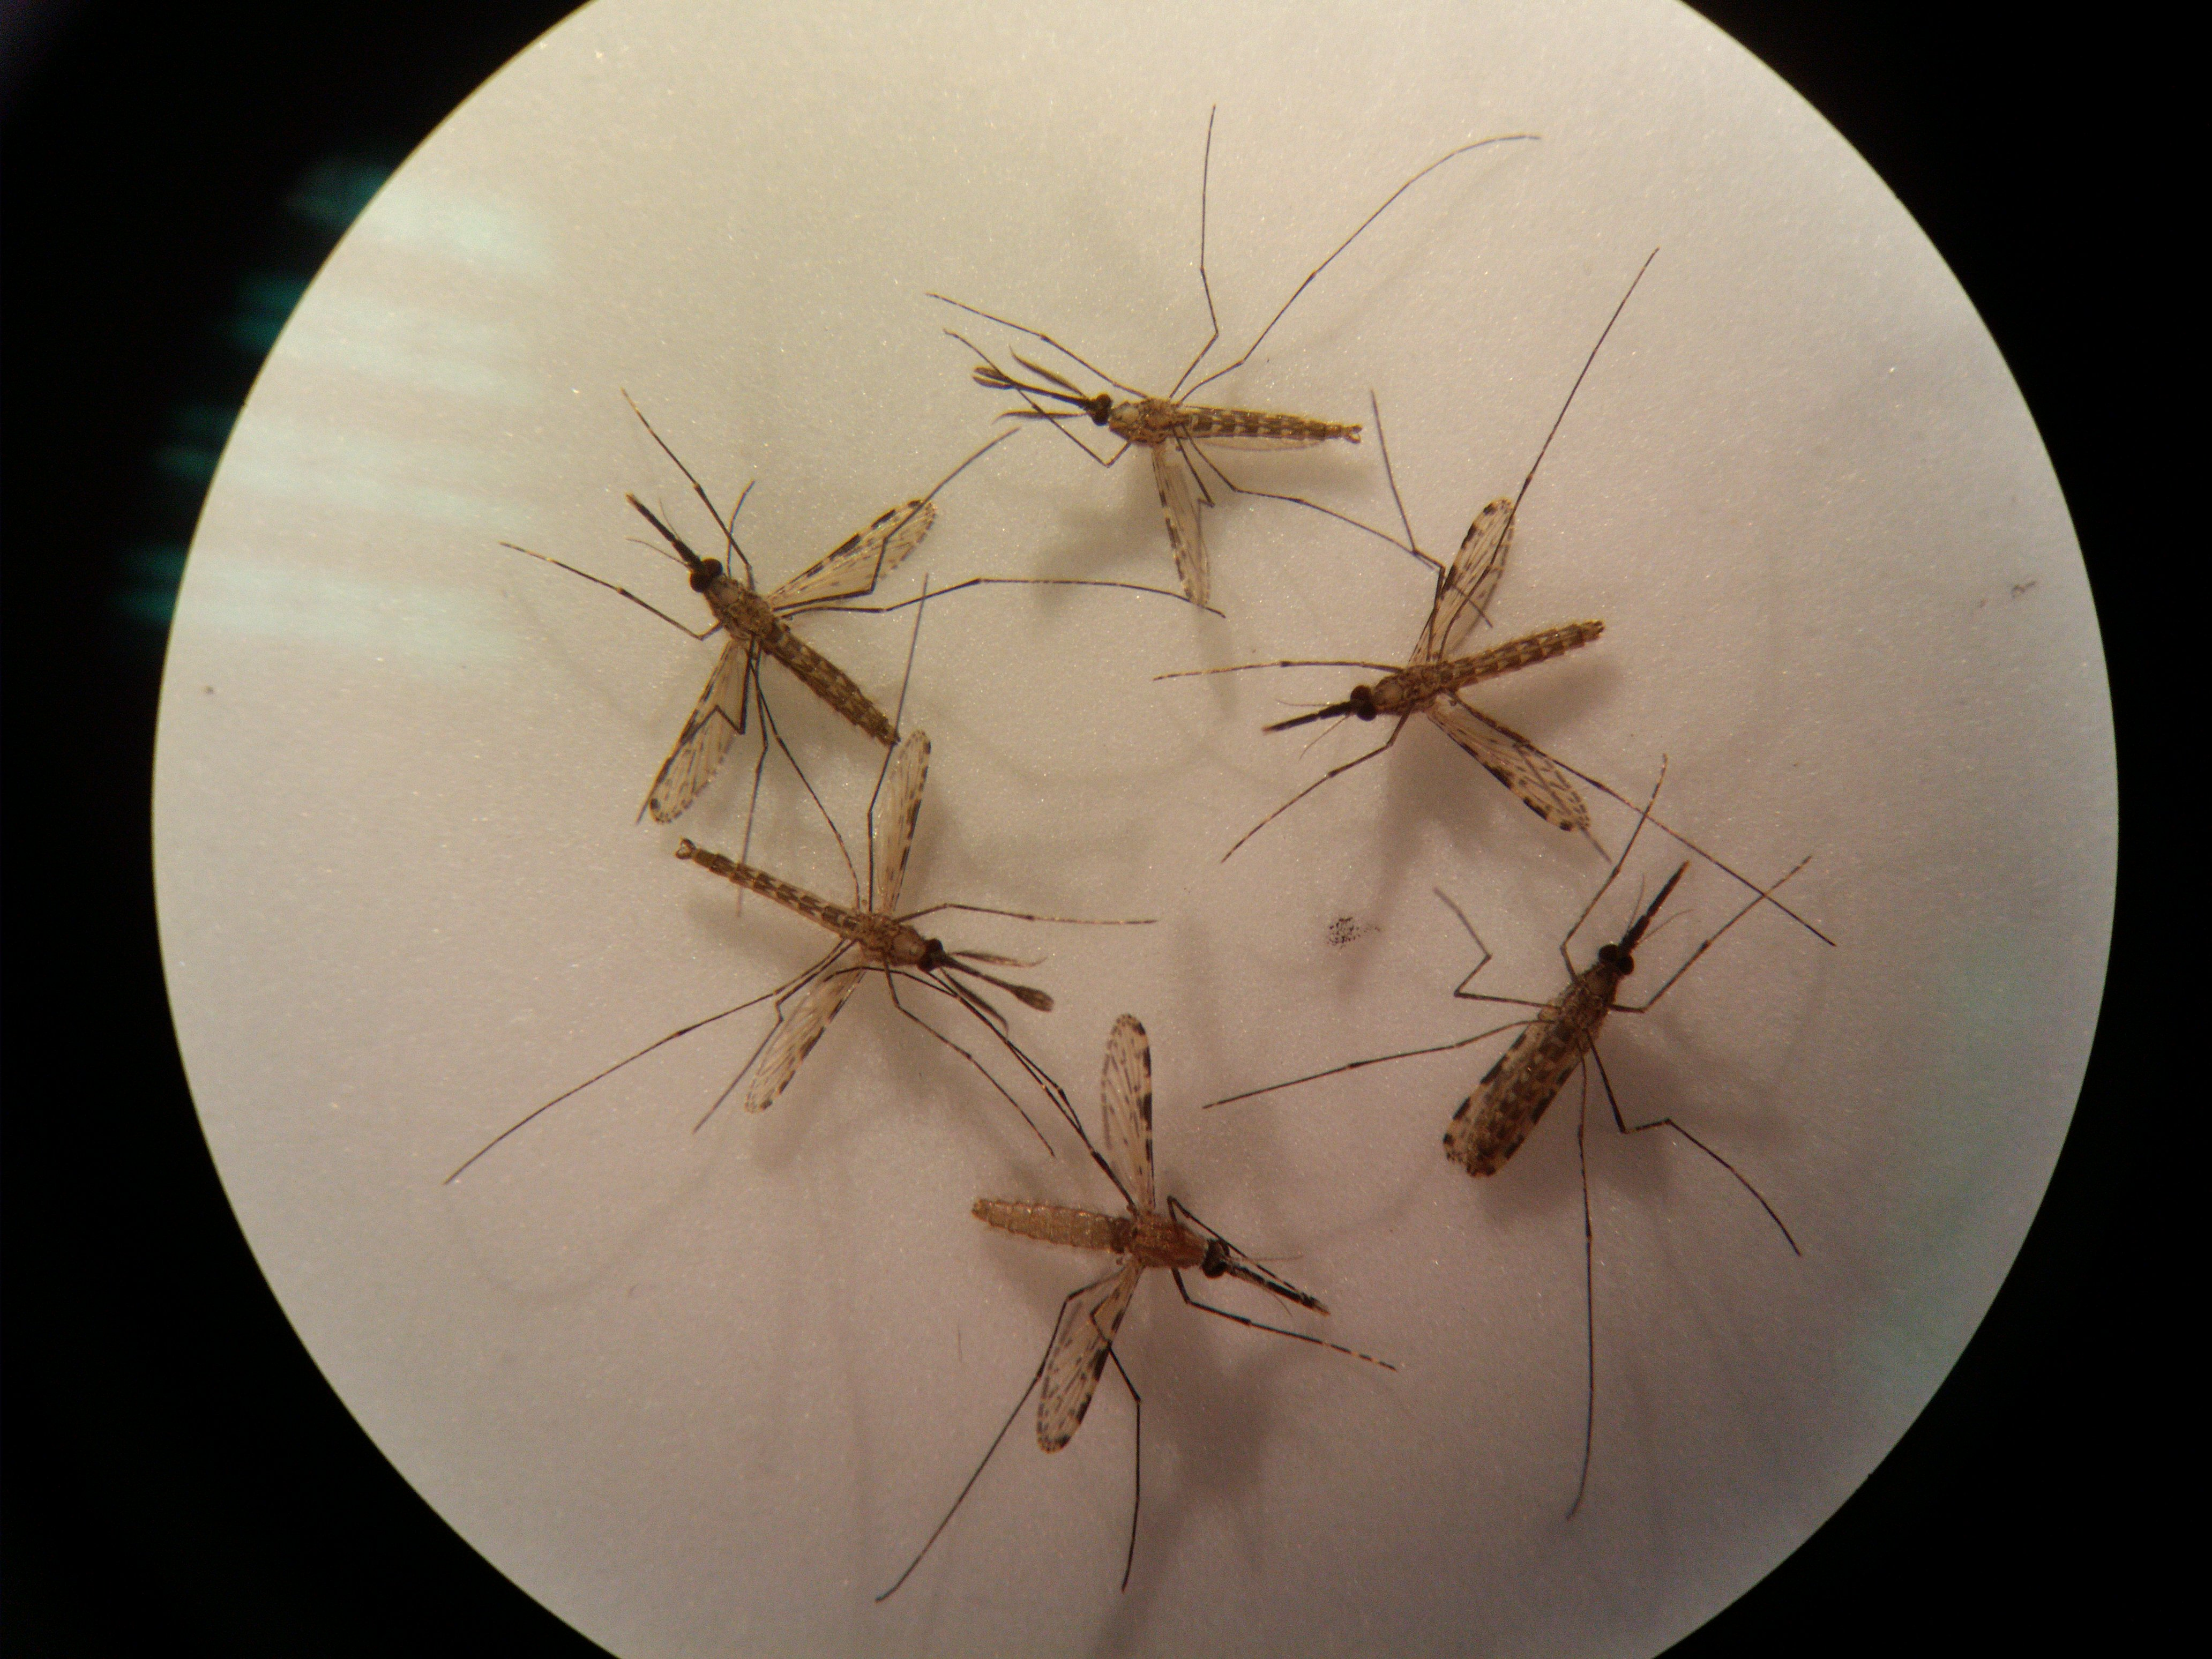
\includegraphics[scale=0.1, angle=90]{mali-NIH-♂_pimp-♀}
\caption{Collected mali-NIH male / pimp female F1 hybrids (4 females, 2 males).}
\label{fig:malimalepimpfemale}
\end{figure}

\begin{figure}[p]
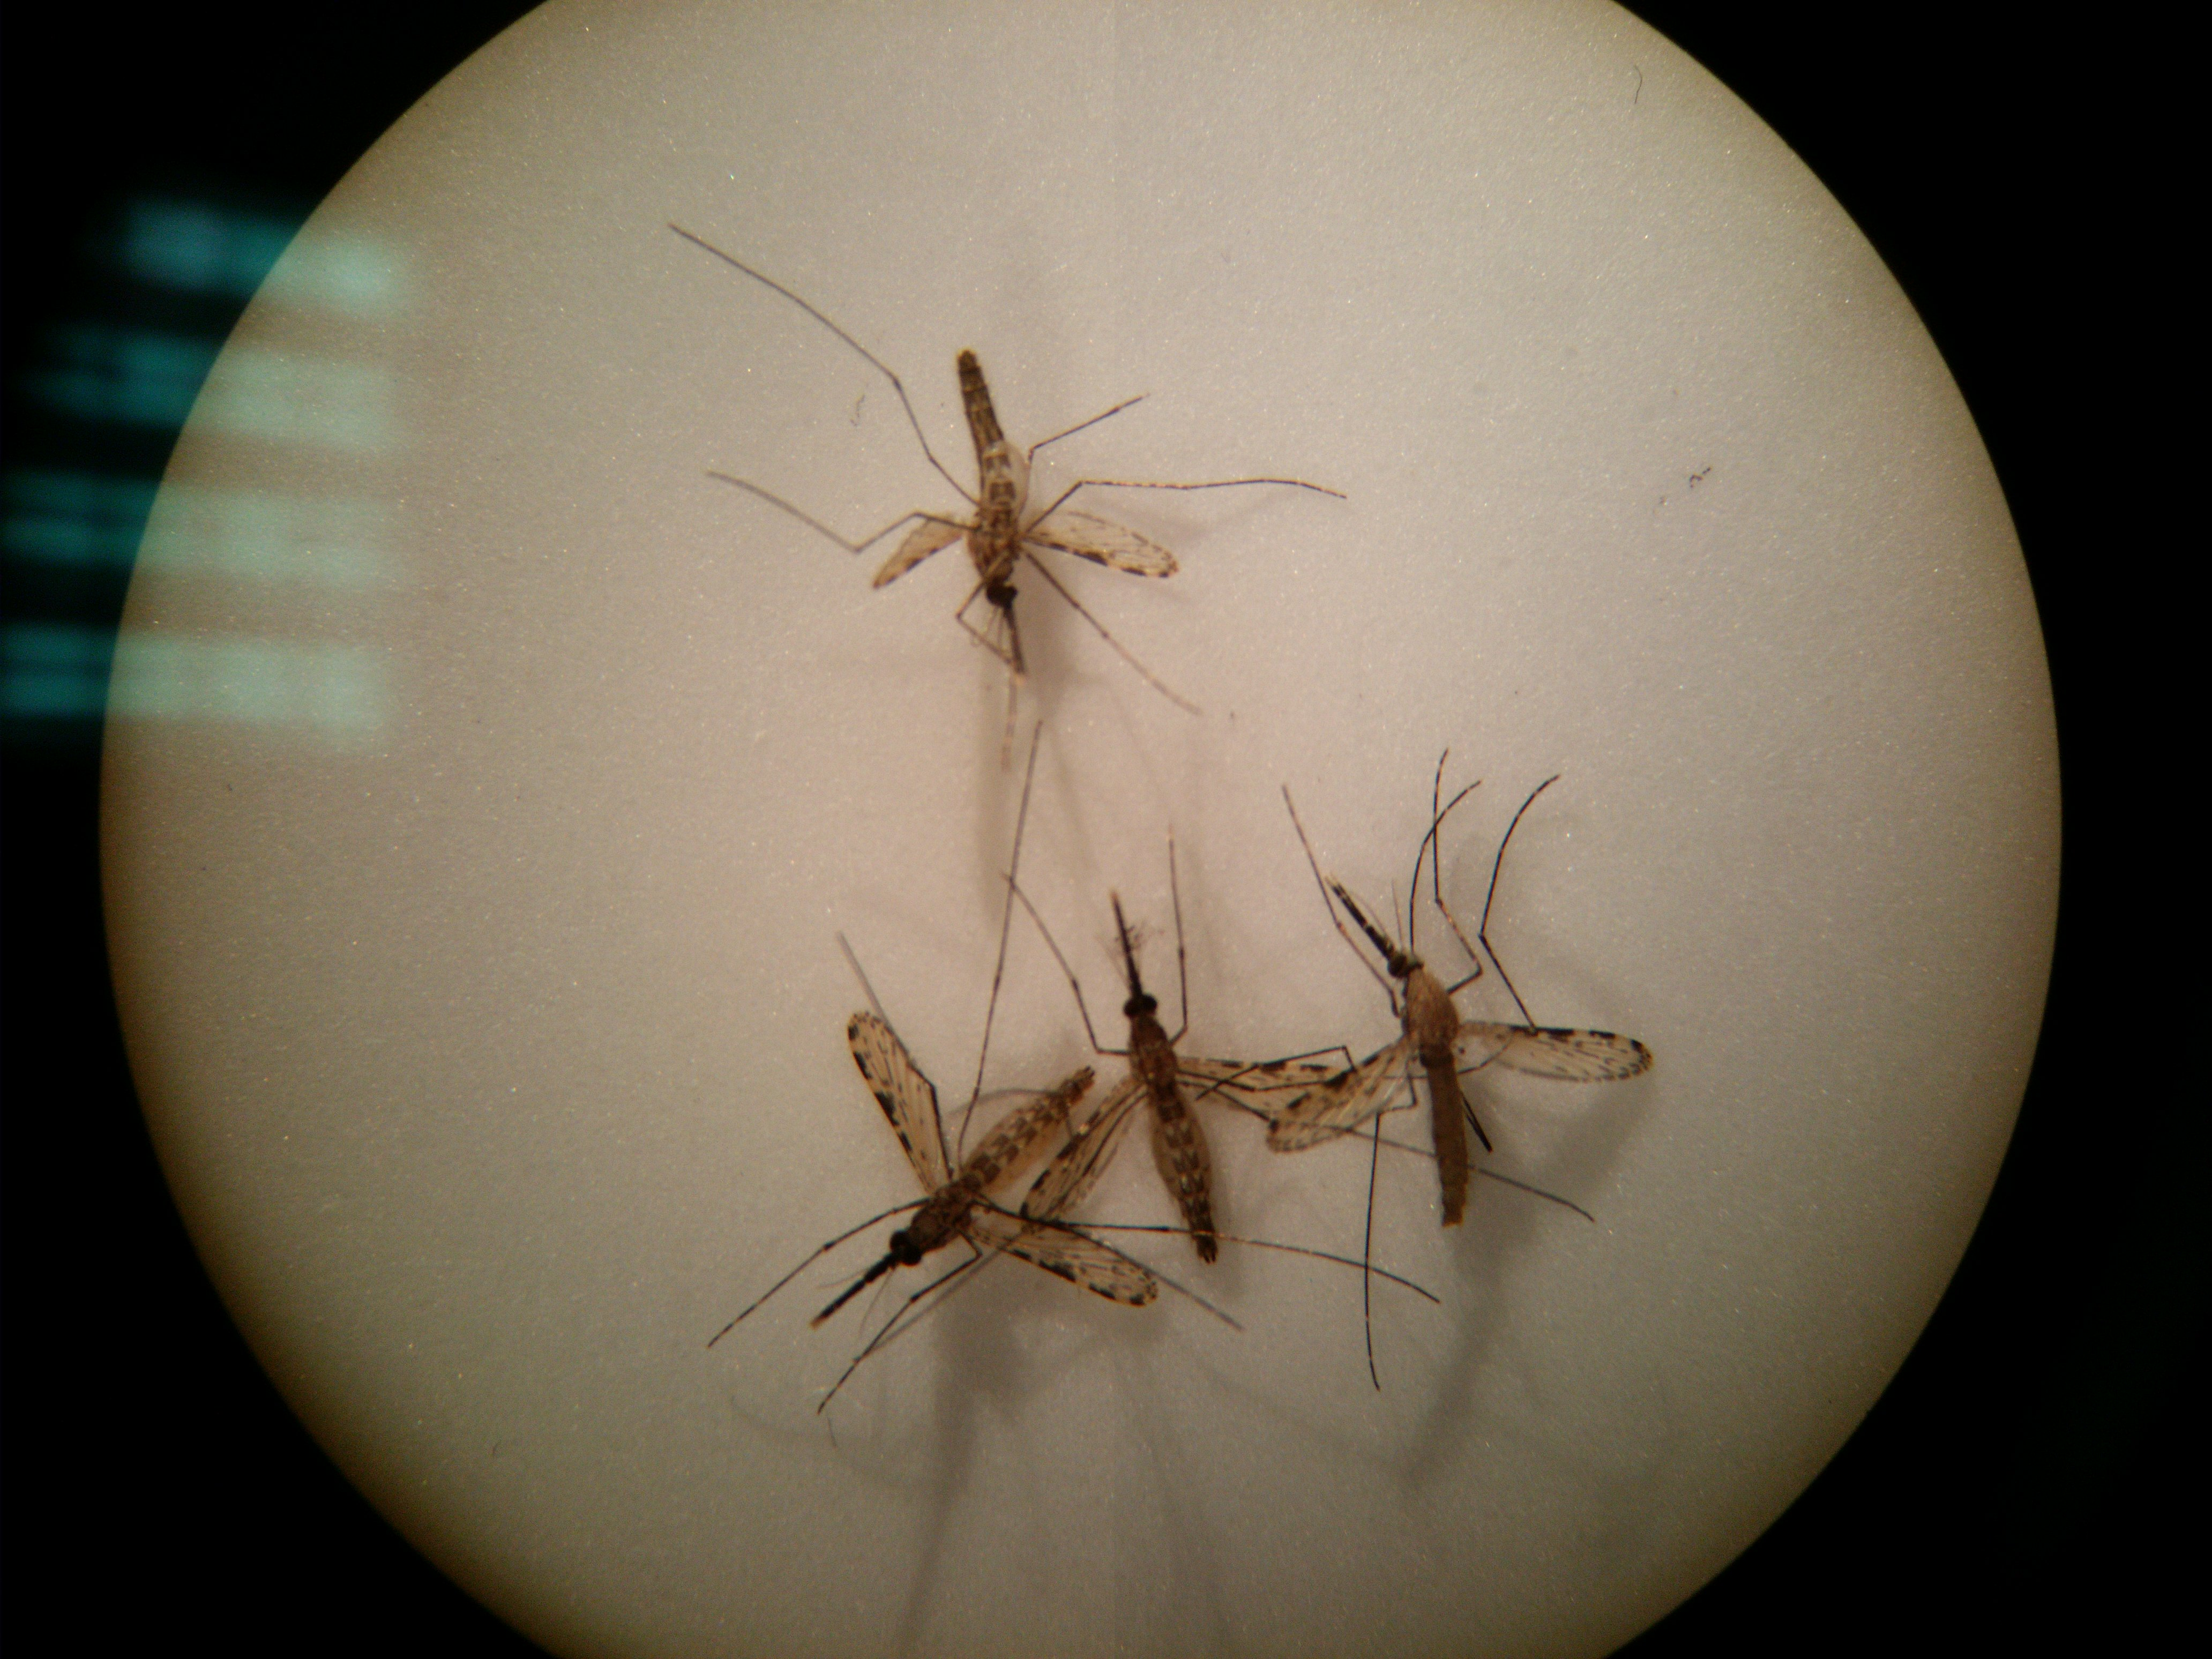
\includegraphics[scale=0.1, angle=90]{pimp-♂_mali-NIH-♀}
\caption{Collected pimp male / mali-nih female F1 hybrids (all are female).}
\label{fig:pimpmalemalifemale}
\end{figure}

\begin{figure}[p]
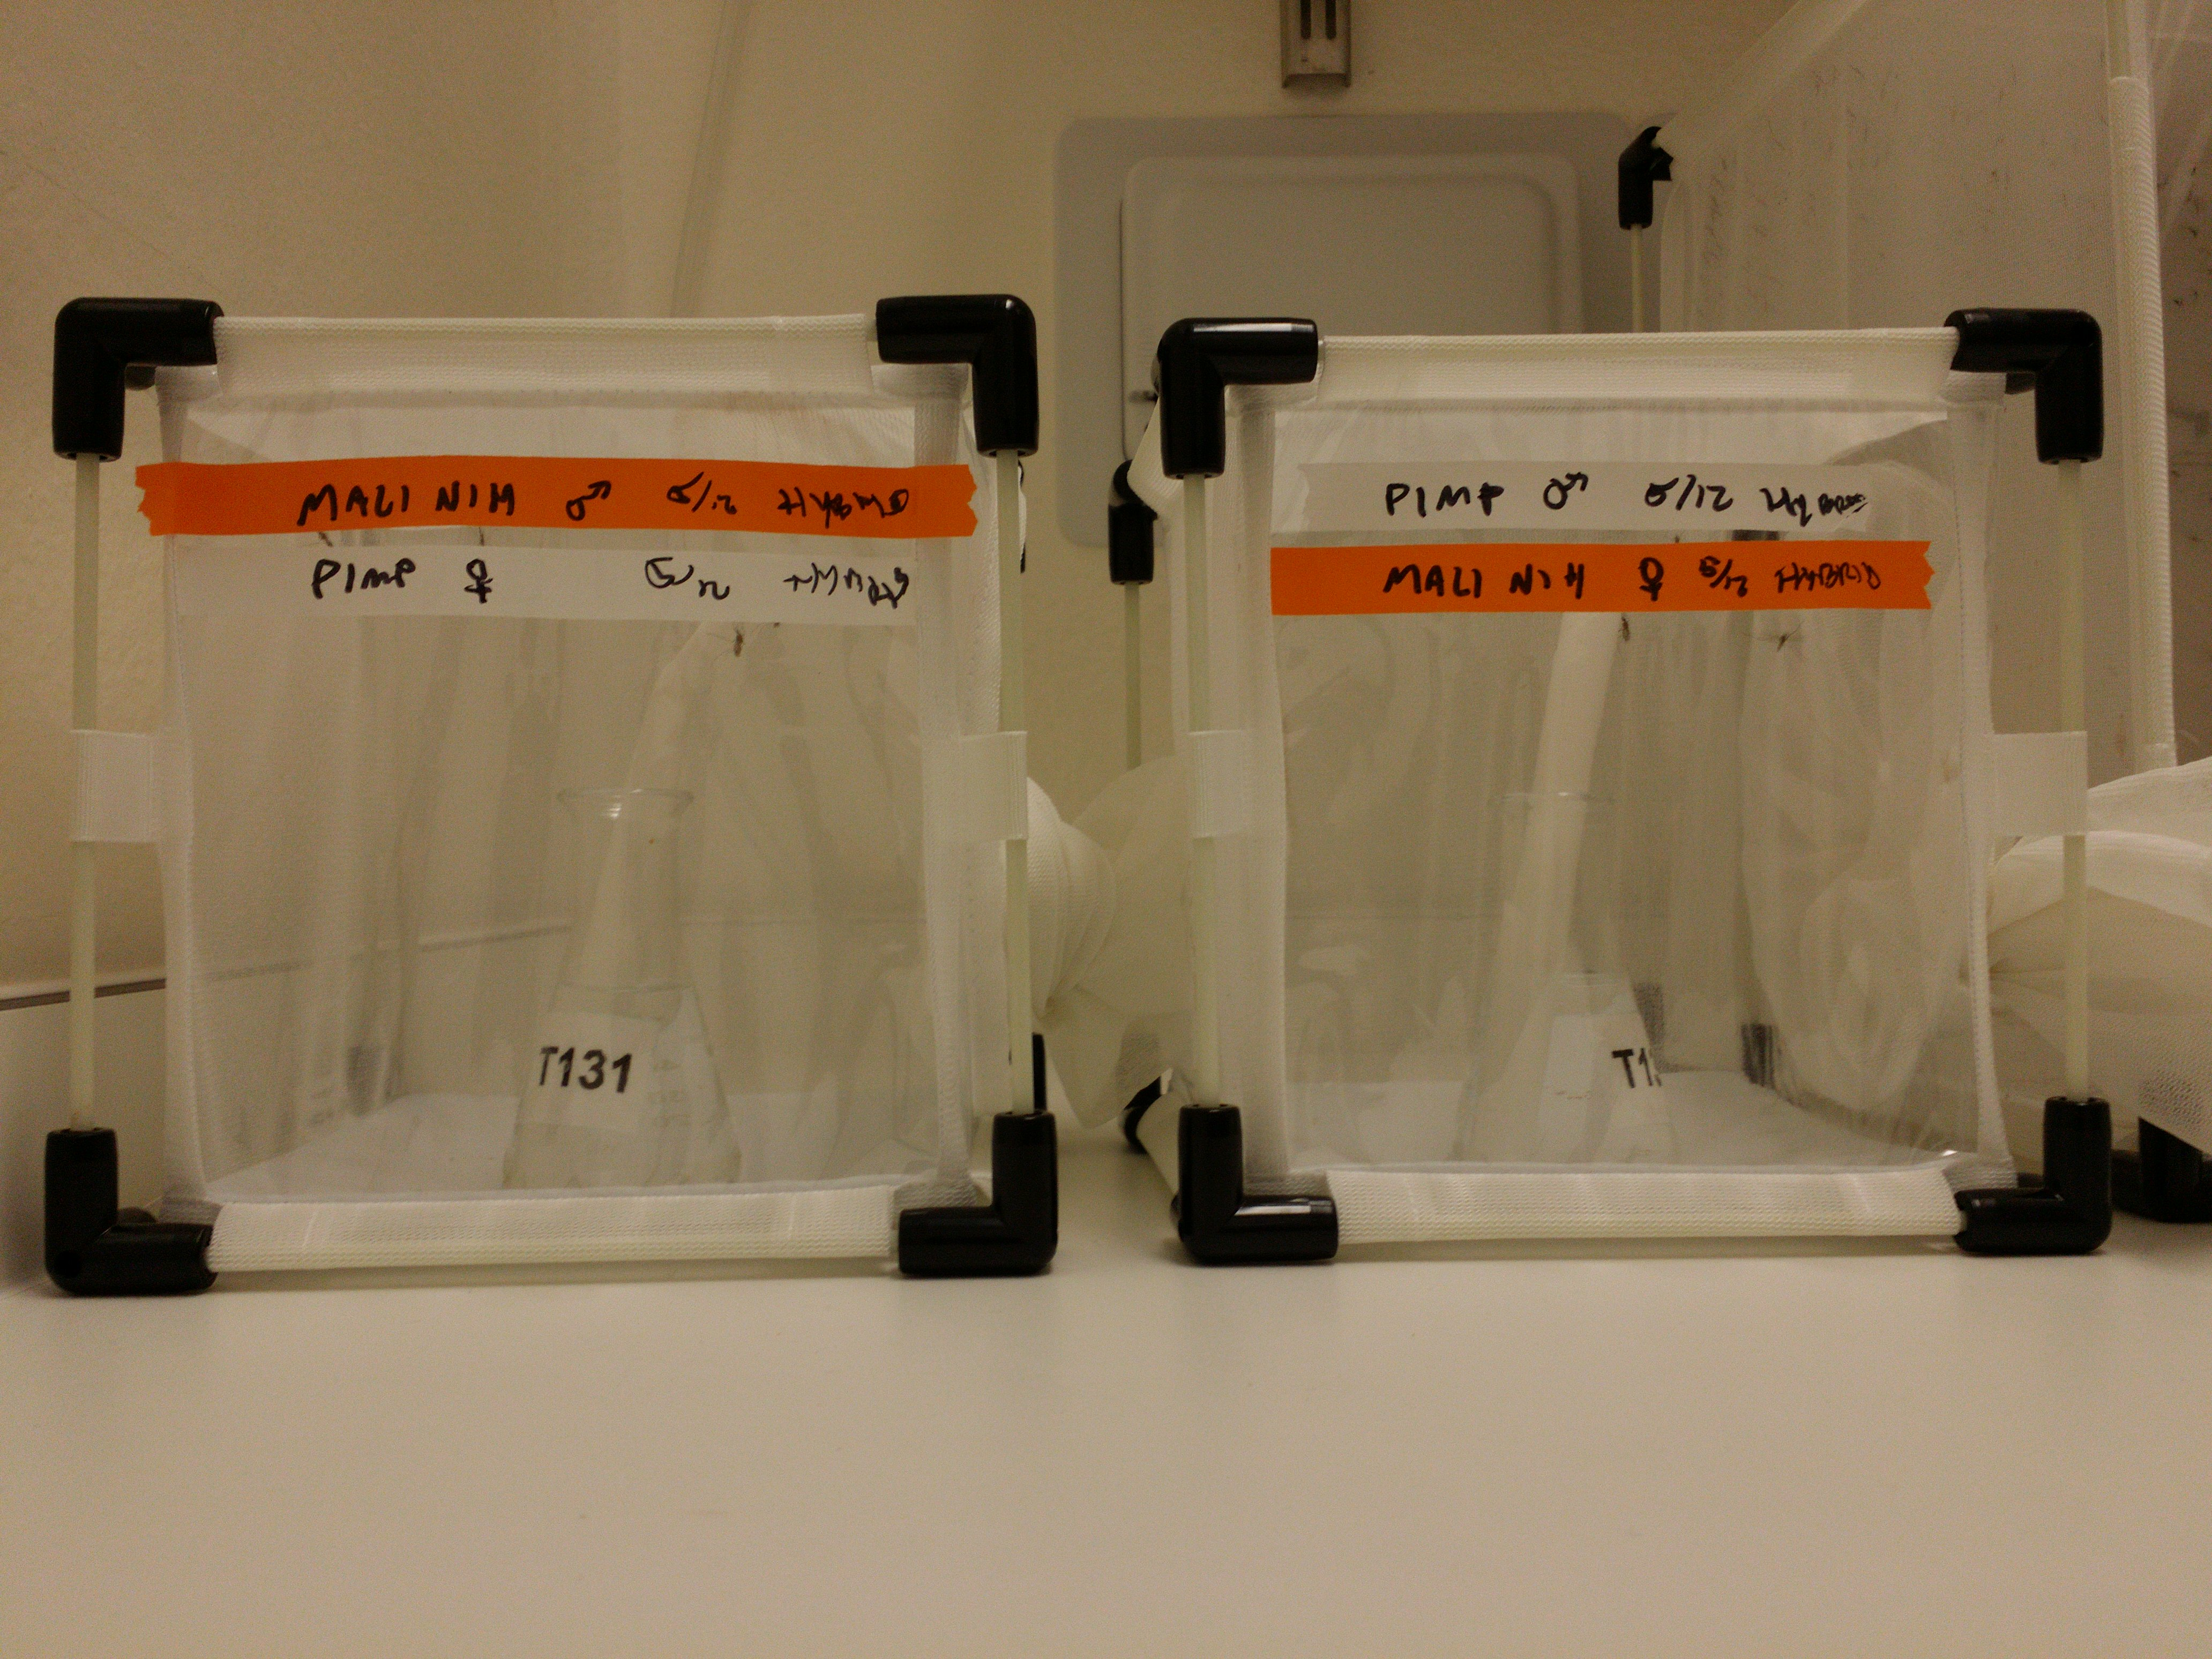
\includegraphics[scale=0.1]{cages}
\caption{Mali-NIH/pimp collection cages. Beakers with filter paper are filled with glucose saturated water provide a source of food for the adult mosquitoes.}
\end{figure}

\begin{figure}[p]
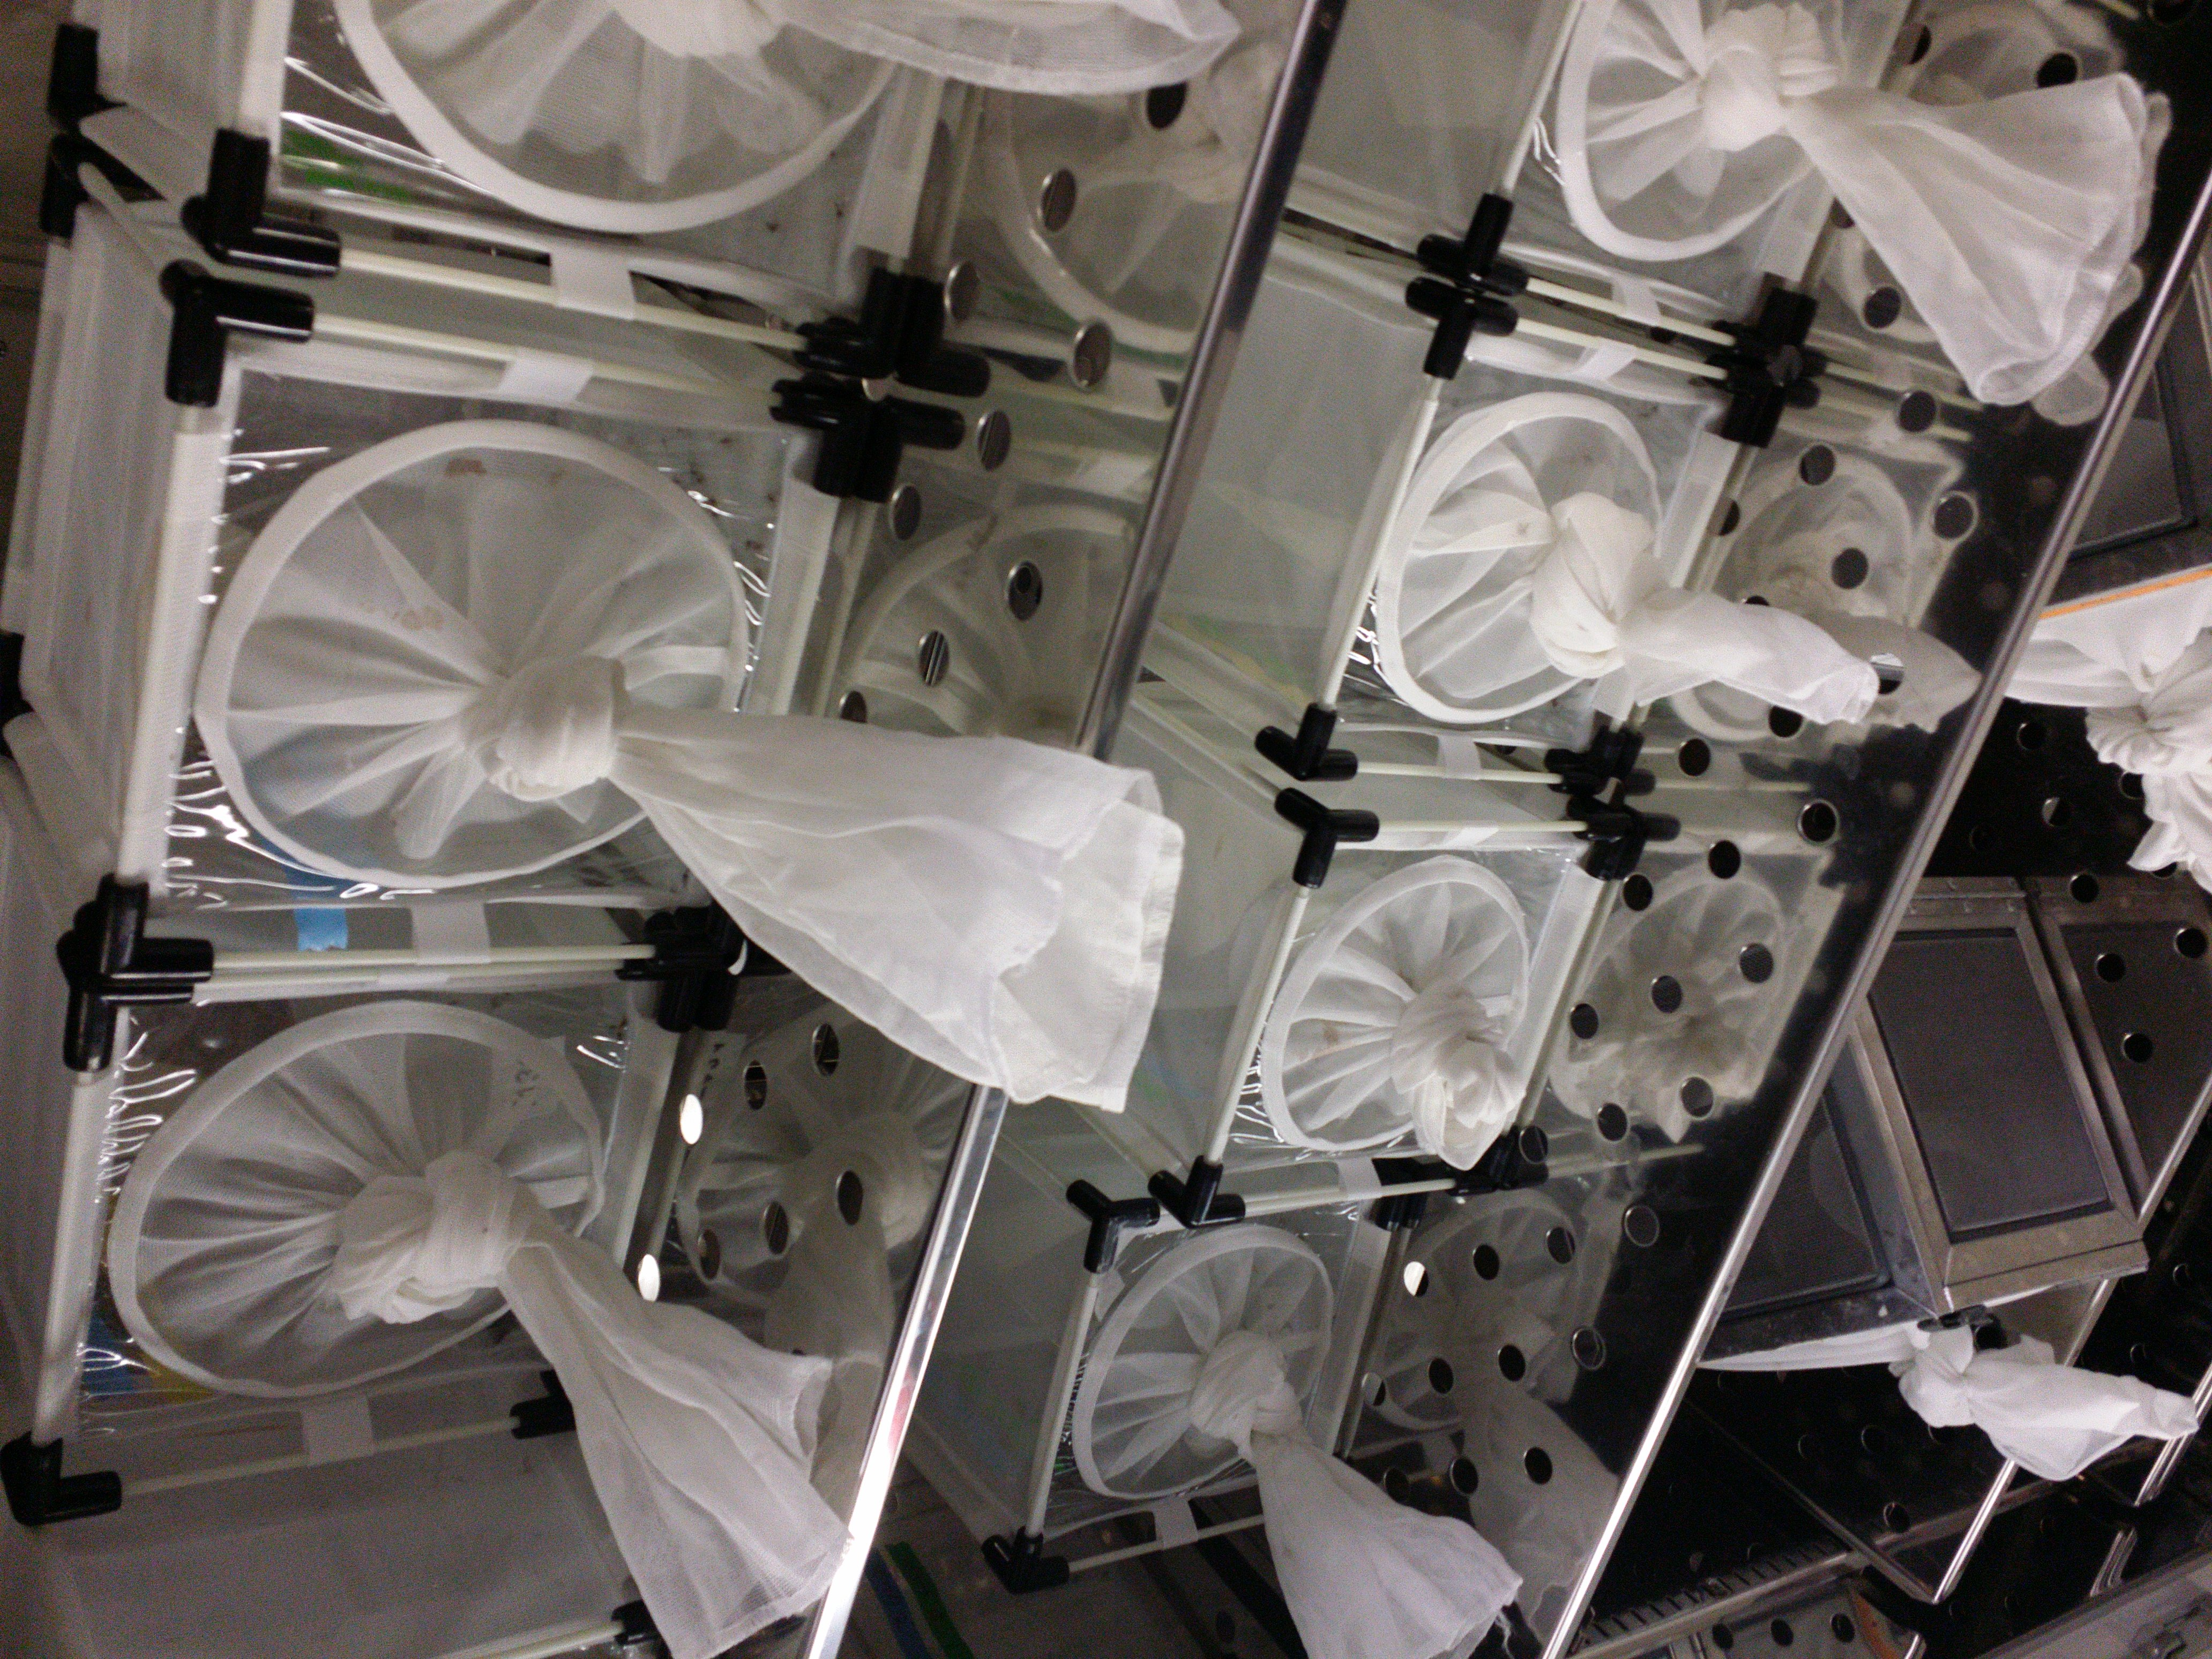
\includegraphics[scale=0.1, angle=270]{allcages}
\caption{Cages from the first phase of the experiment.}
\end{figure}

\begin{figure}[p]
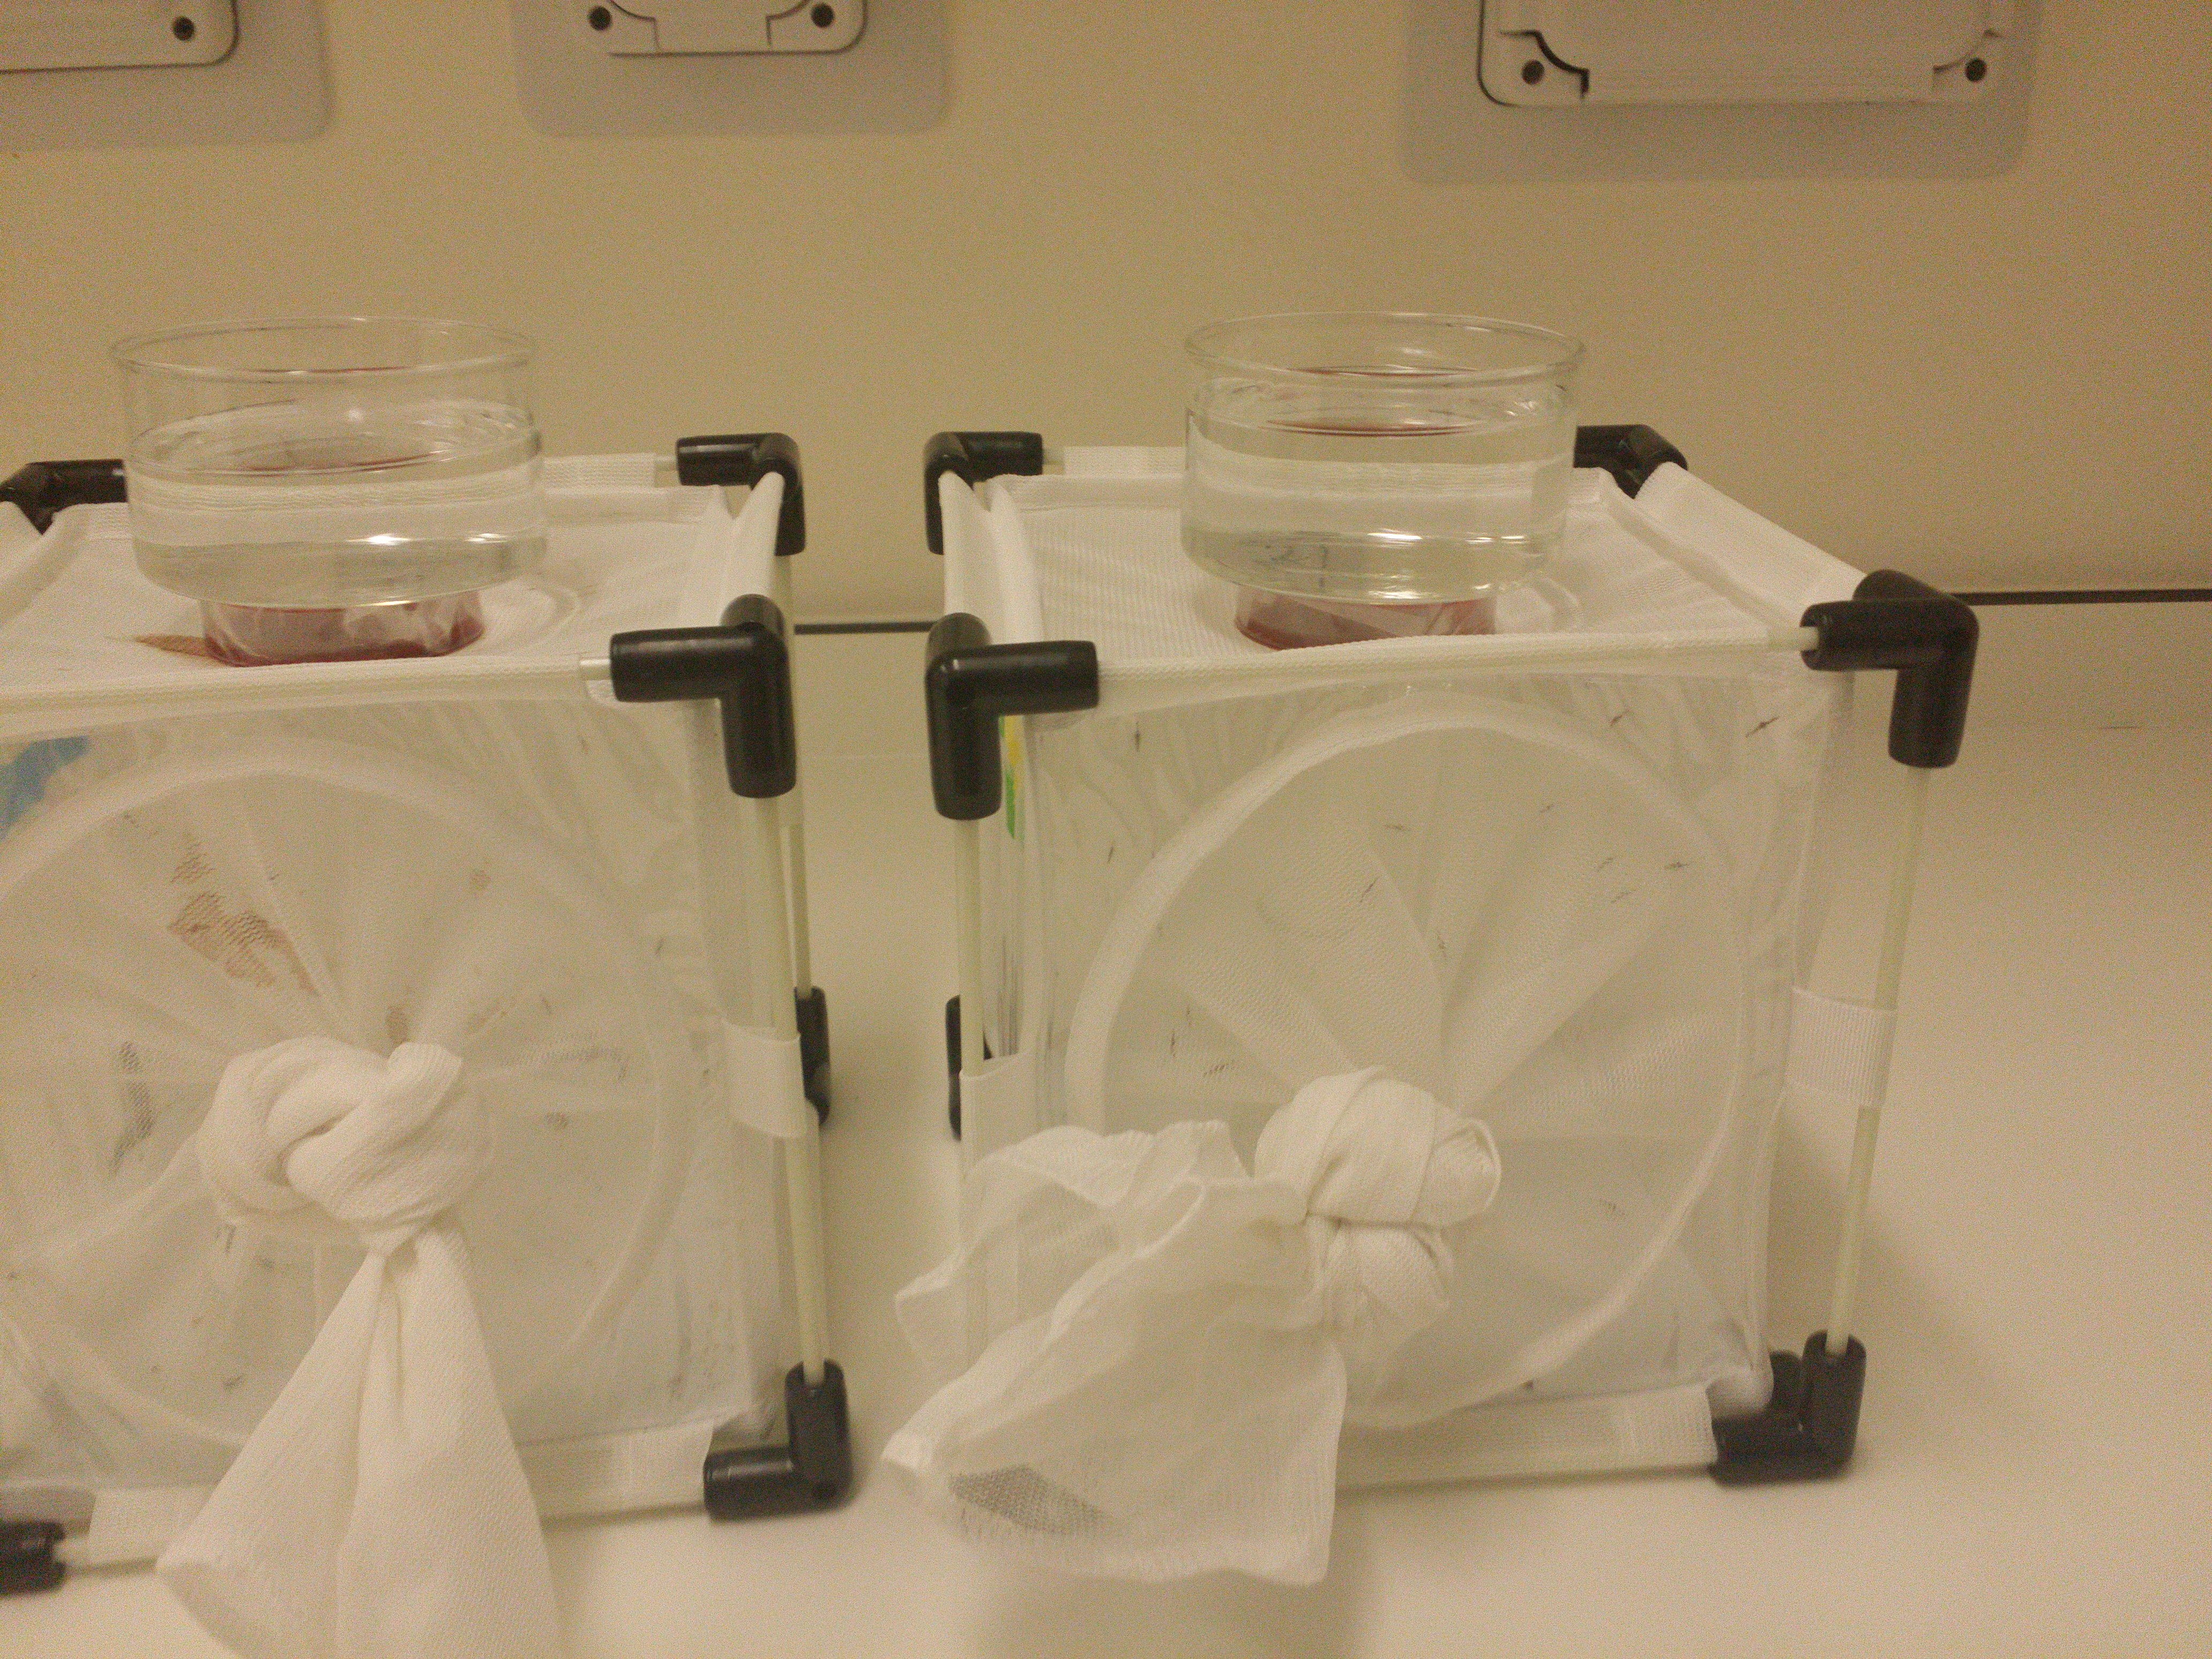
\includegraphics[scale=0.1, angle=0]{feedingsetup}
\caption{Feeding mosquitoes using donor blood. The bood is placed on top of the cages upside down in petri dishes covered by parafilm, while hot water is placed on top of the dishes to simulate the presence of a large mammal and attract female mosquitoes to bite through the parafilm.}
\end{figure}

\begin{figure}[p]
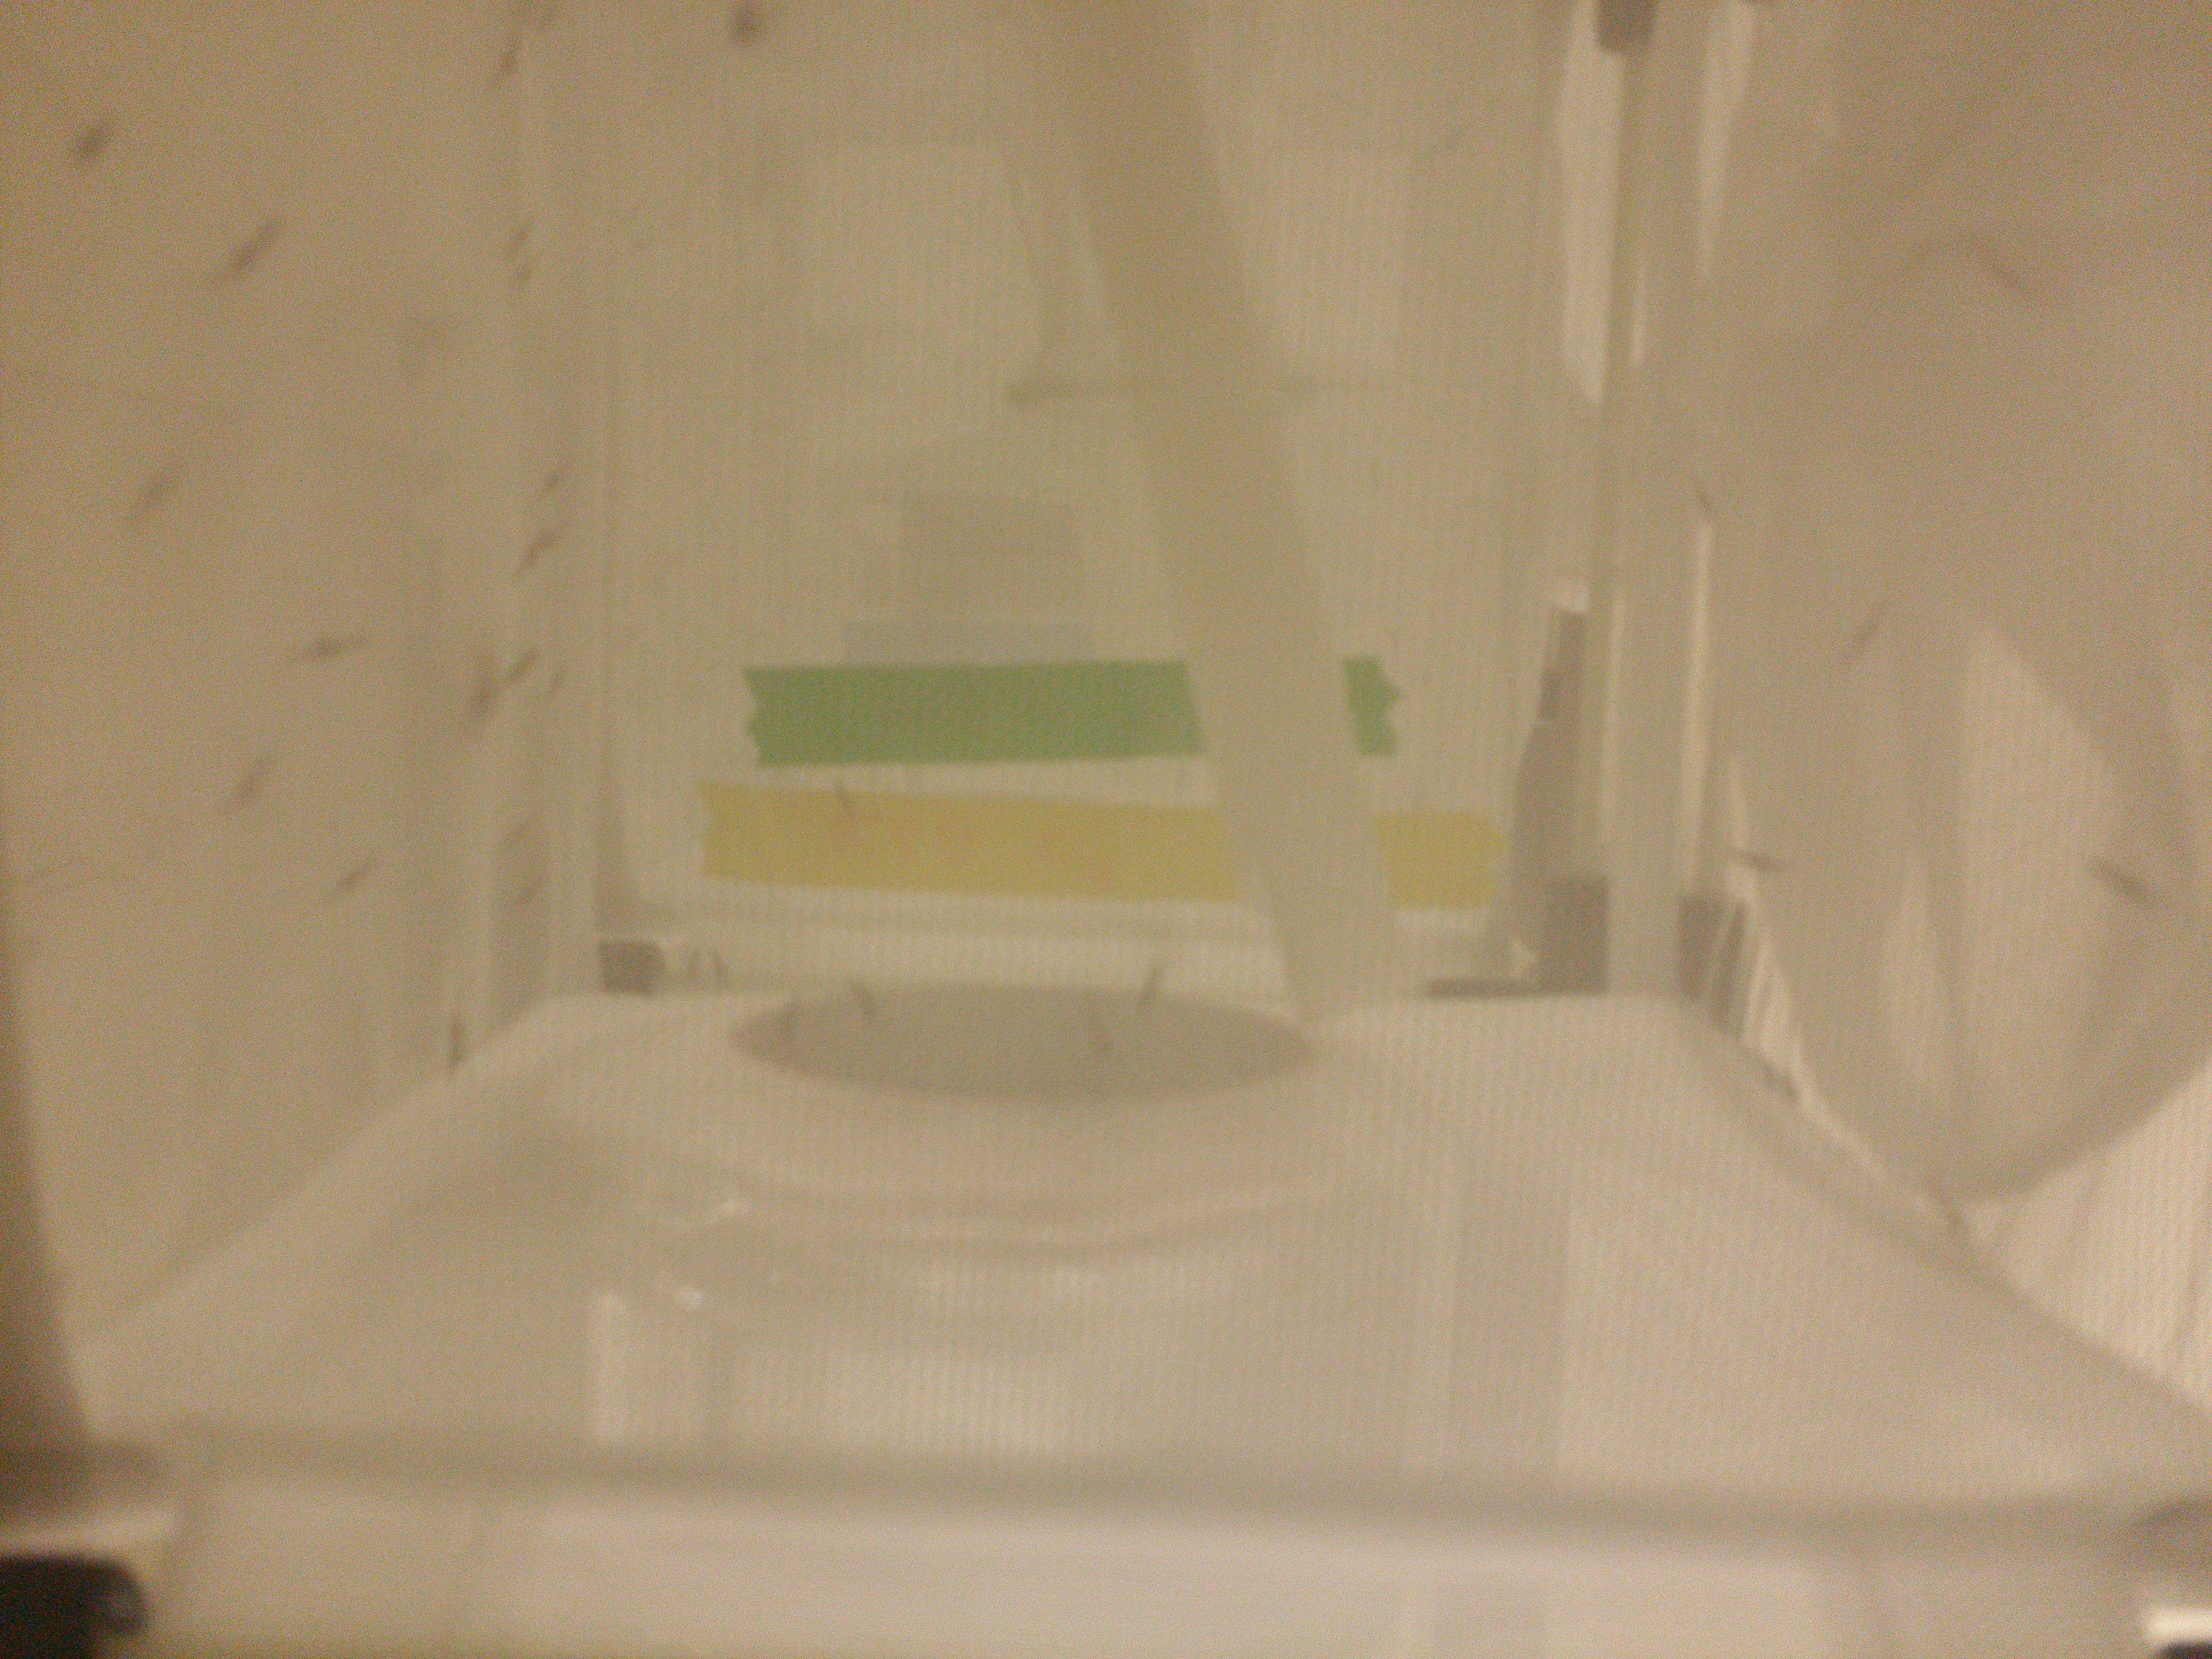
\includegraphics[scale=0.1, angle=180]{feedingmozzies}
\caption{Female mosquitoes feeding on donor blood through netting and parafilm.}
\end{figure}

\end{document}
